\chapter{Записи}
\label{sec:chapter_posts}

\textbf{Записи} (или как их ещё называют — посты) — тип данных, который представляет собой привязанные к дате публикации, отсортированные в обратном хронологическом порядке материалы (новые — сверху, остальные выводятся на следующих страницах).
Записи используются для регулярных публикаций новостей, инструкций, статей, обзоров, отчётов. Список всех записей доступен в меню "Записи / Все записи" (см. рис. \ref{fig:pic_posts}).

\begin{figure}[htp]
    \centering
	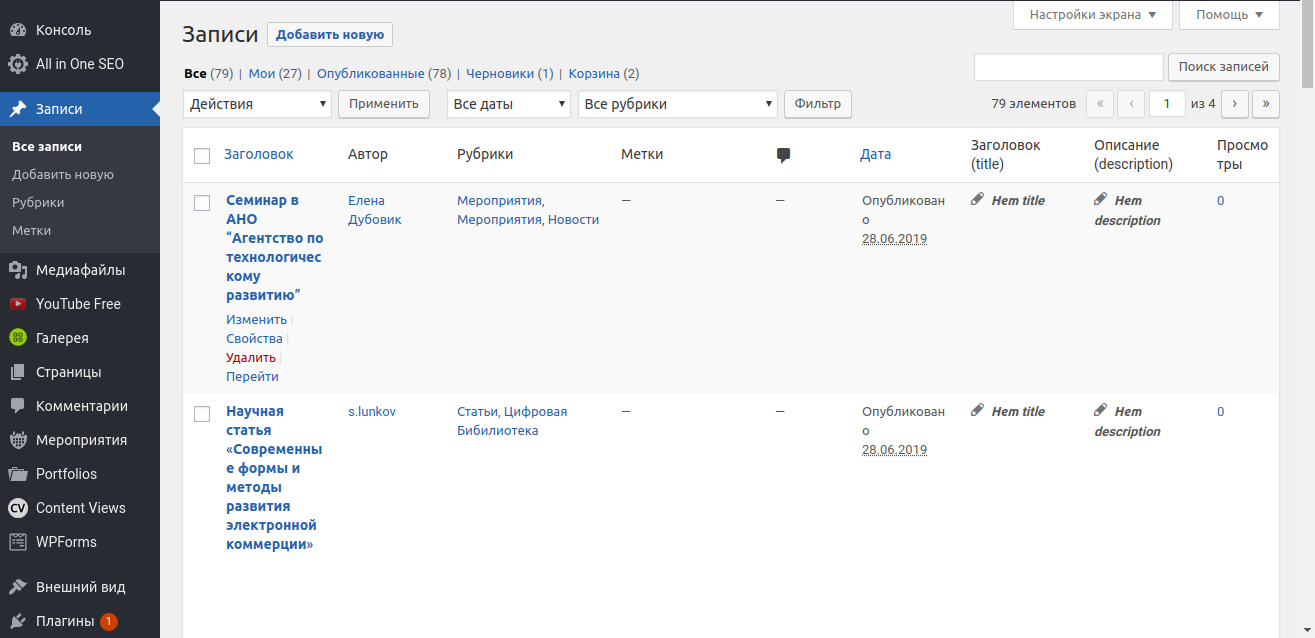
\includegraphics[width=\textwidth]{posts.png}
    \caption{Перечень записей}
    \label{fig:pic_posts}
\end{figure}

\section{Рубрики}
\label{sec:part_cat_posts}

Рубрики дают хорошую возможность группировать связанные записи, а также сообщить читателю, о чём запись. Рубрики также облегчают поиск материалов внутри вашего сайта. Рубрики могут иметь иерархическую структуру, для этого при создании дочерней рубрики установите необходимое значение в поле "Родительская рубрика".
Все записи могут относиться к одной или нескольким рубрикам. Для редактирования рубрик перейдите в меню «Записи / Рубрики» (см. рис. \ref{fig:pic_posts_cat})

\begin{figure}[htp]
    \centering
	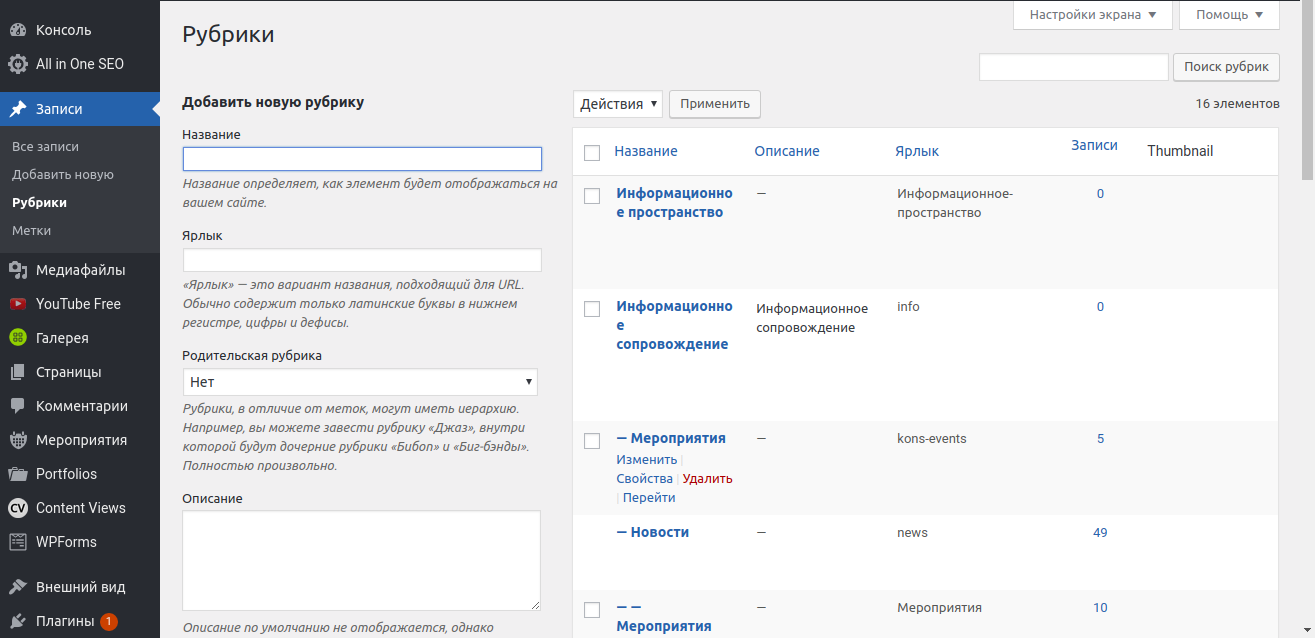
\includegraphics[width=\textwidth]{posts_cat.png}
    \caption{Рубрики»}
    \label{fig:pic_posts_cat}
\end{figure}


\section{Создание новой записи}
\label{sec:part_new_post}

Для публикации изображения к новости, перейдите в низ страницы раздел «Изображение записи» (см. рис. ниже)




Выберите изображение из медиа-библиотеки (см. рис. ниже)




После установки изображения нажмите кнопку «Опубликовать» (вверху страницы).


Нажмите кнопку «Добавить слайд» и в появившемся окне выберите изображение (см. рис. ниже)


Для каждого изображения в слайдере можно добавить описание. Для сохранения изменений в слайдере нажмите кнопку «Сохранить»

